\pdfminorversion=4
\documentclass[aspectratio=169]{beamer}

\mode<presentation>
{
  \usetheme{default}
  \usecolortheme{default}
  \usefonttheme{default}
  \setbeamertemplate{navigation symbols}{}
  \setbeamertemplate{caption}[numbered]
  \setbeamertemplate{footline}[frame number]  % or "page number"
  \setbeamercolor{frametitle}{fg=white}
  \setbeamercolor{footline}{fg=black}
} 

\usepackage[english]{babel}
\usepackage[utf8x]{inputenc}
\usepackage{tikz}
\usepackage{courier}
\usepackage{array}
\usepackage{bold-extra}
\usepackage{minted}
\usepackage[thicklines]{cancel}
\usepackage{fancyvrb}

\xdefinecolor{dianablue}{rgb}{0.18,0.24,0.31}
\xdefinecolor{darkblue}{rgb}{0.1,0.1,0.7}
\xdefinecolor{darkgreen}{rgb}{0,0.5,0}
\xdefinecolor{darkgrey}{rgb}{0.35,0.35,0.35}
\xdefinecolor{darkorange}{rgb}{0.8,0.5,0}
\xdefinecolor{darkred}{rgb}{0.7,0,0}
\definecolor{darkgreen}{rgb}{0,0.6,0}
\definecolor{mauve}{rgb}{0.58,0,0.82}

\title[2018-09-18-jlab-reprise]{Data analysis tools from within HEP and from industry}
\author{Jim Pivarski}
\institute{Princeton University -- DIANA-HEP}
\date{September 18, 2018}

\usetikzlibrary{shapes.callouts}

\begin{document}

\logo{\pgfputat{\pgfxy(0.11, 7.4)}{\pgfbox[right,base]{\tikz{\filldraw[fill=dianablue, draw=none] (0 cm, 0 cm) rectangle (50 cm, 1 cm);}\mbox{\hspace{-8 cm}
\includegraphics[height=1 cm]{princeton-logo-long.png}
\includegraphics[height=1 cm]{diana-hep-logo-long.png}}}}}

\begin{frame}
  \titlepage
\end{frame}

\logo{\pgfputat{\pgfxy(0.11, 7.4)}{\pgfbox[right,base]{\tikz{\filldraw[fill=dianablue, draw=none] (0 cm, 0 cm) rectangle (50 cm, 1 cm);}\mbox{\hspace{-8 cm}
\includegraphics[height=1 cm]{princeton-logo.png}
\includegraphics[height=1 cm]{diana-hep-logo.png}}}}}

% Uncomment these lines for an automatically generated outline.
%\begin{frame}{Outline}
%  \tableofcontents
%\end{frame}

% START START START START START START START START START START START START START

\begin{frame}{The point I want to make}
\large
\vspace{0.5 cm}
\begin{itemize}\setlength{\itemsep}{0.25 cm}
\item Although nuclear and high energy physics once dealt with the world's largest datasets, this is no longer true. ``Big Data'' or (better) ``Web Scale'' analysis regularly deals with petabytes and exabytes, and they've developed software tools for it.

\item<2-> We can reduce maintenance costs and improve students' career options by mixing industry standard tools with our in-house tools, particularly for cases in which the purpose of the tool is the same.

\item<3-> This is in line with ROOT's new Python and TMVA interfaces, but broader: data should flow freely to the best tool for the job and back again, leaving the choice in the physicist's hands.
\end{itemize}

\uncover<4->{\textcolor{darkblue}{In short, we should become like other sciences, like astronomy or biology: common libraries for common stuff and our own libraries for domain-specific stuff.}}
\end{frame}

\begin{frame}{\only<1>{We measure globally distributed data in hundreds of PB}\only<2>{But for ``web scale'' companies, 100 PB = 1 truck}}
\vspace{0.35 cm}
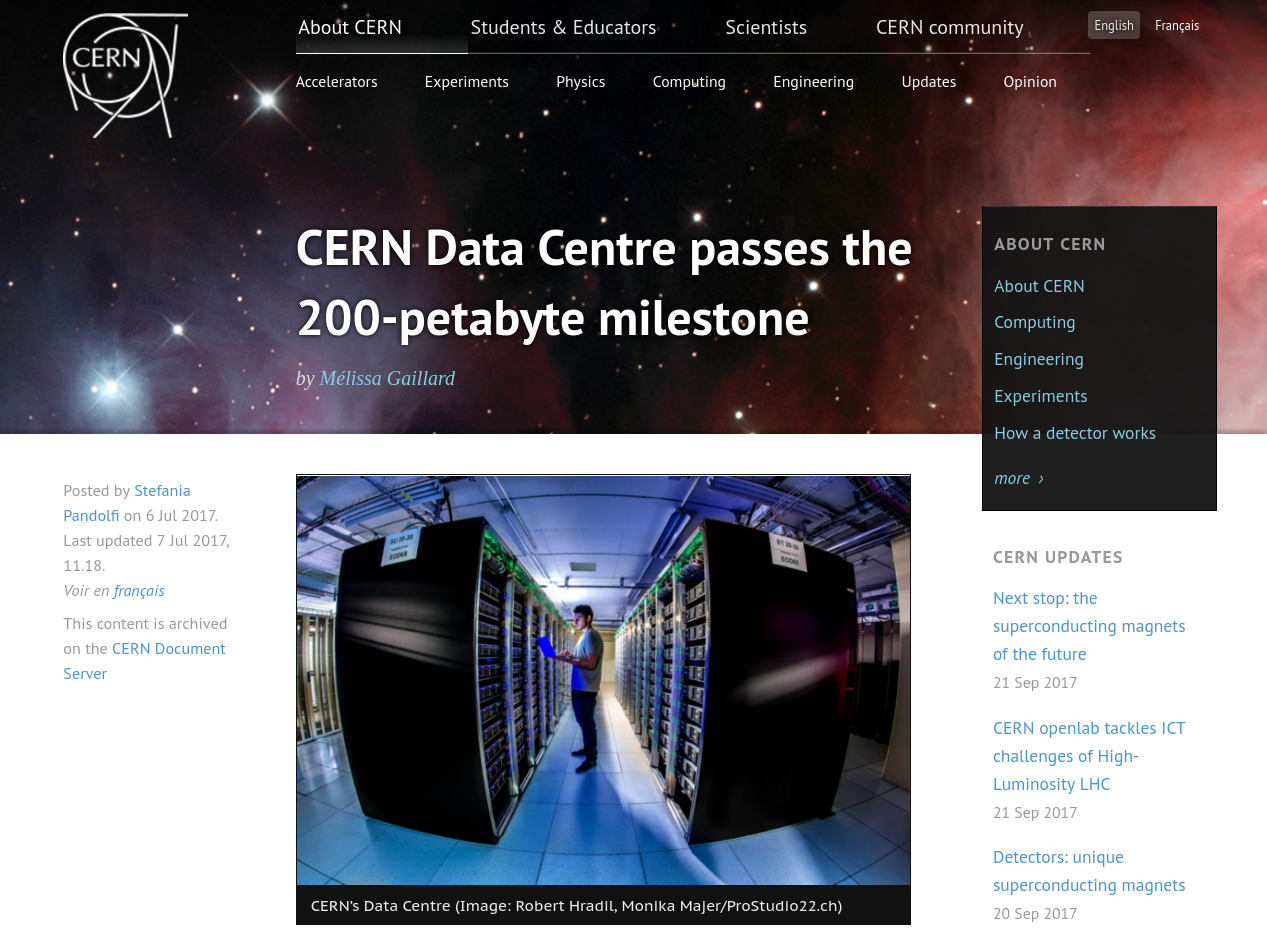
\includegraphics[width=0.73\linewidth]{cern-200pb.png}

\vspace{-4.8 cm}
\uncover<2->{\mbox{ } \hfill 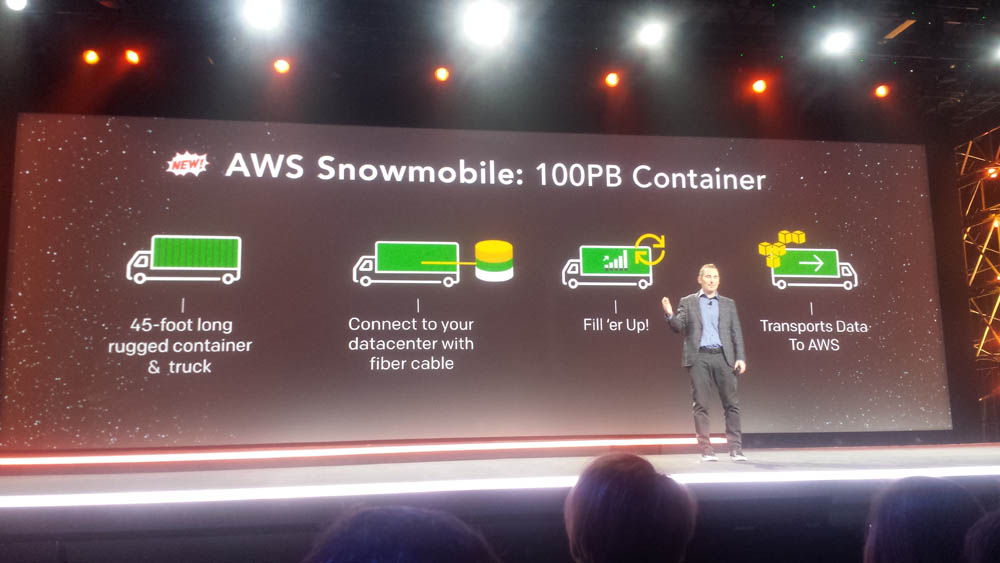
\includegraphics[width=0.7\linewidth]{aws-snowmobile.jpg}\hspace{-1 cm}}
\end{frame}

\begin{frame}{Number of people (users and developers) also dwarf our field}
\vspace{0.25 cm}
\mbox{ } \hfill 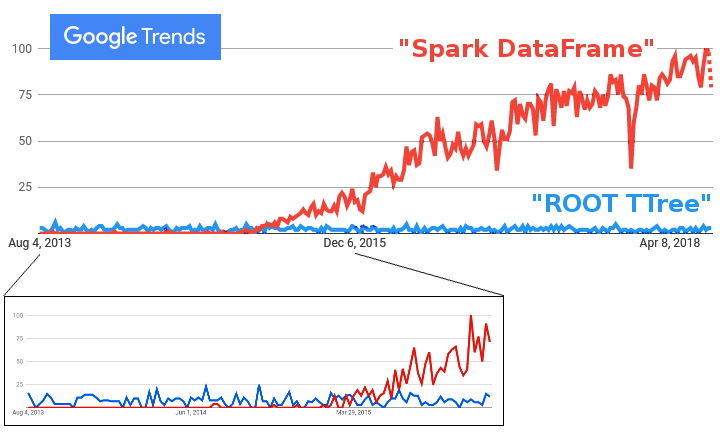
\includegraphics[width=0.9\linewidth]{root-spark-google-trends.png} \hfill \mbox{ }
\end{frame}

\begin{frame}{Number of people (users and developers) also dwarf our field}
\large
\vspace{0.5 cm}
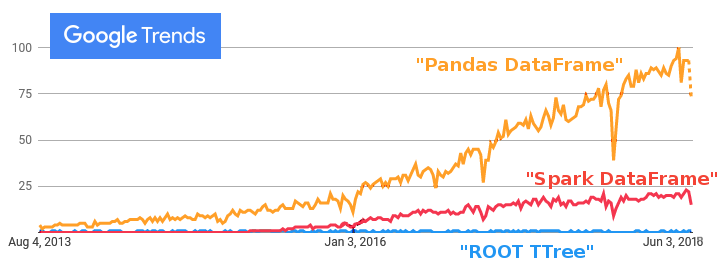
\includegraphics[width=\linewidth]{root-spark-pandas-google-trends.png}

\vspace{0.5 cm}
\uncover<2->{More users means more bug reports, more online help, more how-to blogs\ldots}

\vspace{0.2 cm}
\uncover<2->{More developers means more bug-fixes, more features, more connectors\ldots}
\end{frame}



\end{document}
